\section{Deep Learning}

\begin{frame}{Project Data to solve complex tasks}
    \note{Deep learning relies on several key principles that enable it to effectively learn from complex data}
  

    \begin{center}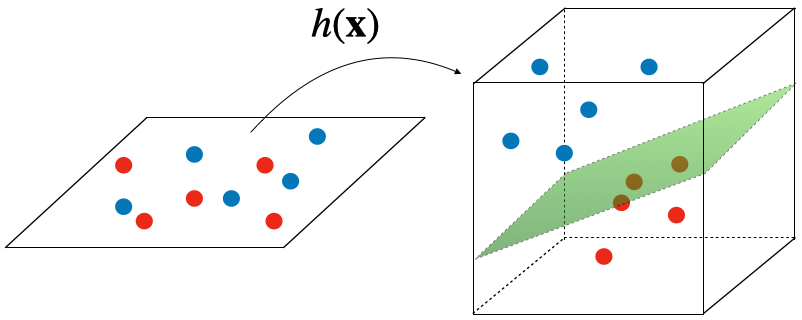
\includegraphics[width=200px]{img/projection.png}\end{center}
    \vspace{0.5cm}
    \begin{itemize}
        \note{Consequence of Cover's theorem (computational learning theory): set of training data that is not linearly separable, can with high probability be transformed into a training set that is linearly separable by projecting it into a higher-dimensional space via some non-linear transformation}
        \item A complex pattern-classification problem, cast in a high-dimensional space nonlinearly, is more likely to be linearly separable than in a low-dimensional space, provided that the space is not densely populated (Cover's theorem).
        \item Primary theoretical motivations for the use of non-linear kernel methods in ML (Poynomial and Radial Basis Function kernels in SVM)
    \end{itemize}
  
  
  \end{frame}

  \begin{frame}{Deep Learning}  

    \begin{textblock}{40}(65, 20)
        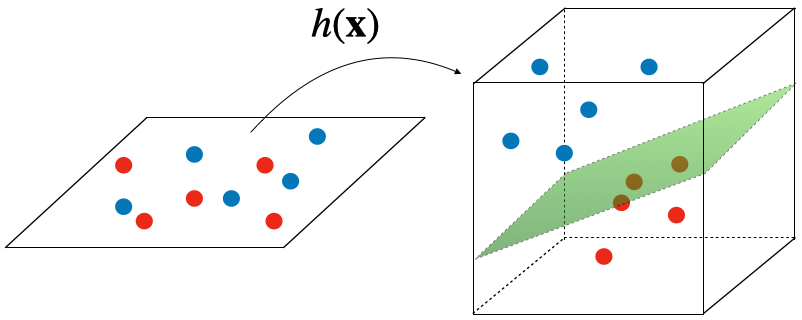
\includegraphics[width=110px]{img/projection.png}
    \end{textblock}
    \begin{textblock}{40}(65, 40)
      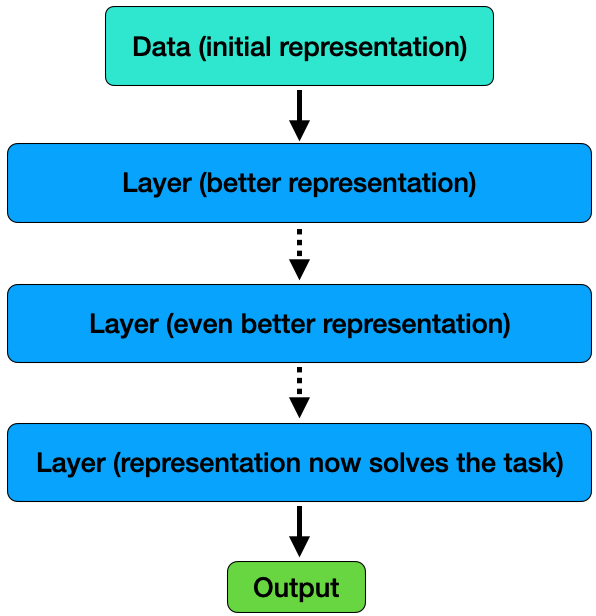
\includegraphics[width=120px]{img/projection_dl.png}
    \end{textblock}

    
    \begin{textblock}{60}(1, 15)
        \begin{itemize}
            \item Deep learning is the subset of machine learning methods based on Neural Networks (NN)
            \item NN model learns a complex non-linear function that will project the data in a high-dimension space where the data are linearly separable or where we have a better representation of the data to solves the task
            \item To do so, NN model project the data non-linearly successively through several neural layers improving representation at each step
            \item The adjective "deep" refers to the use of multiple layers in the network
          \end{itemize}
    \end{textblock}
  
  
  \end{frame}

\begin{frame}{Deep Learning}
  \begin{textblock}{60}(1, 15)
    \begin{itemize}
      \item These layers performs operations which either:
      \begin{itemize}
        \item Project non-linearly (typically linear-layer + non linear activation function)
        \item Capture the structural patterns and relationships within the data (Convolutional layers in Convolutional Neural Network (CNN), Attention mechanisms in Transformers, Aggregation functions in Graph Neural Network (GNN))
      \end{itemize}
      \item The combination of non-linear projections and the capture of structural patterns allows neural network models to learn complex non-linear functions, projecting data into a space where their representations can solve the task effectively
      \item Two examples: The transformers and the GNNs
    \end{itemize}
  \end{textblock}

  \begin{textblock}{40}(65, 20)
    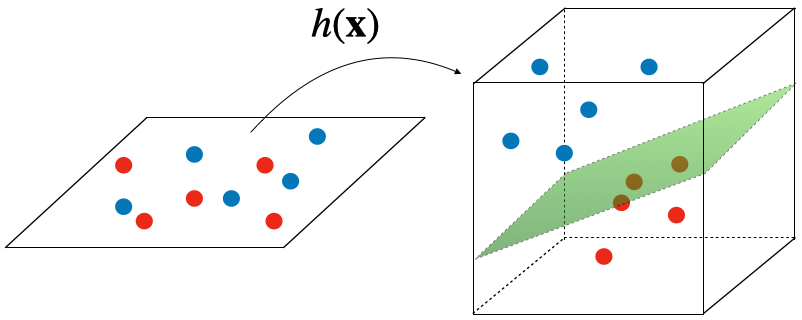
\includegraphics[width=110px]{img/projection.png}
  \end{textblock}
  \begin{textblock}{40}(65, 40)
    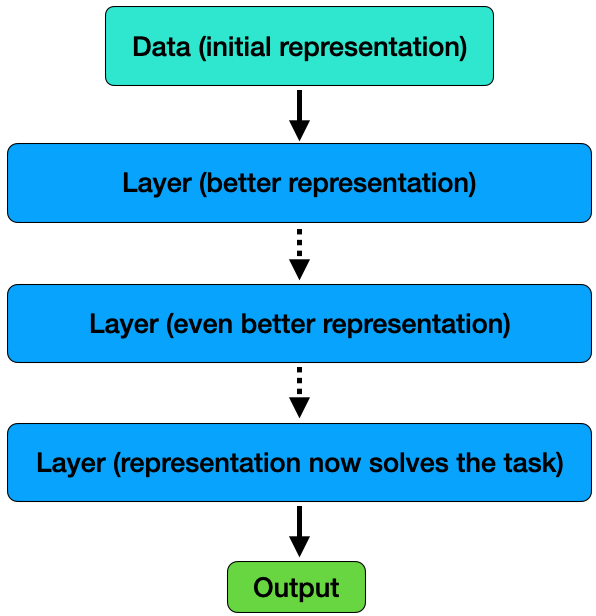
\includegraphics[width=120px]{img/projection_dl.png}
  \end{textblock}

\end{frame}


%\subsection{A few example}

\begin{frame}{Transformers}
  \begin{itemize}
      \item We hear it all the time: Large Language Models (LLMs) predict "only" the next word in a sentence, the most likely word.
      \item That's true. But the real question is how do LLMs do it??
      \item To answer this question, we need to understand the architectures on which they are based: Transformers and their core mechanism: the attention mechanism
  \end{itemize}
\end{frame}


\begin{frame}{Transformers}
    \begin{itemize}
        \item Transformers are a type of model architecture primarily used in the field of natural language processing (NLP)
        \item They have become foundational for tasks such as translation, text generation, text summarization, and sentiment analysis
        \item Introduced in the seminal paper "Attention is All You Need" in 2017, transformers represent a significant shift from previous Recurrent Neural Network models approachs in NLP
      \end{itemize}
\end{frame}

\begin{frame}{Transformers}
    \begin{textblock}{50}(2, 15)
        Goal: identify and attend to most important features in input that are relevant to the semantic meaning
    \end{textblock}
    \begin{textblock}{48}(2, 35)
        \setbeamercovered{transparent}

        \onslide<1->{1. Input \textbf{embeddings}}

        \onslide<2->{2. Encode \textbf{position} information}

        \onslide<3->{3. Compute 3 independant linear projection: \textbf{query, key, value}}

        \onslide<6->{4. Compute \textbf{attention weighting}}   
        
        \onslide<10->{5. Ponderate value features with \textbf{attention scores}}

        %\onslide<11->{These operations form a self attention head.}

        %\onslide<11->{Multi head attention : Multiple head attend on different type of complex relationship in the input sequence.}


    \end{textblock}

    \begin{textblock}{48}(52, 25)
        \includegraphics<1>[width=150px]{img/transformer_1.png}
        \includegraphics<2>[width=150px]{img/transformer_2.png}
        \includegraphics<3>[width=150px]{img/transformer_3.png}
        \includegraphics<4>[width=150px]{img/transformer_4.png}
        \includegraphics<5>[width=150px]{img/transformer_5.png}
        \only<6-9>{Attention score: compute pairwise similarity between each query and key}
        \only<6-7>{How compute similarity between vectors of features?}
        \includegraphics<7>[width=150px]{img/transformer_6.png}
        \includegraphics<8>[width=150px]{img/transformer_7.png}
        \includegraphics<9>[width=150px]{img/transformer_8.png}
        \includegraphics<10>[width=150px]{img/transformer_9.png}
    \end{textblock}

\end{frame}

\begin{frame}{Transformers: Attention Mechanisms}
  \begin{textblock}{60}(2, 15)
    \textbf{Scaled Dot-Product Attention} : \\  
    
    \[
    \text{Attention}(Q, K, V) = \text{softmax}\left(\frac{QK^T}{\sqrt{d_k}}\right)V
    \]

    These operations form a self-attention head that can plug into a larger network.\\ 
  \end{textblock}
  \begin{textblock}{60}(2, 52)
    \textbf{Multi-Head Attention} : \\
    We can multiply the attention head to enhance the model's ability by allowing it to capture different type of relationship between the element of the sequence
    \[
    \text{MultiHead}(Q, K, V) = \text{Concat}(\text{head}_1, \ldots, \text{head}_h)W^O
    \]
    where $\text{head}_i = \text{Attention}(QW_i^Q, KW_i^K, VW_i^V)$
  \end{textblock}

  \begin{textblock}{38}(62, 15)
    \begin{center}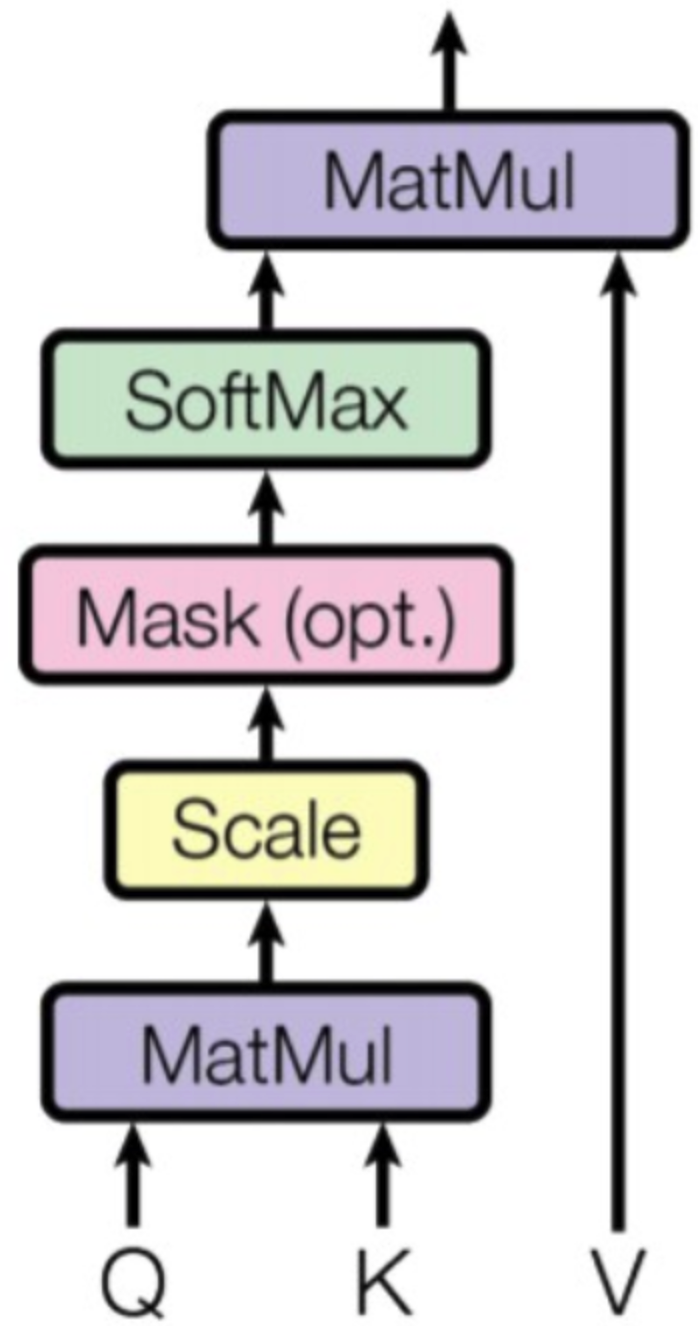
\includegraphics[width=40px]{img/transformer_10.png}\end{center}
    \begin{center}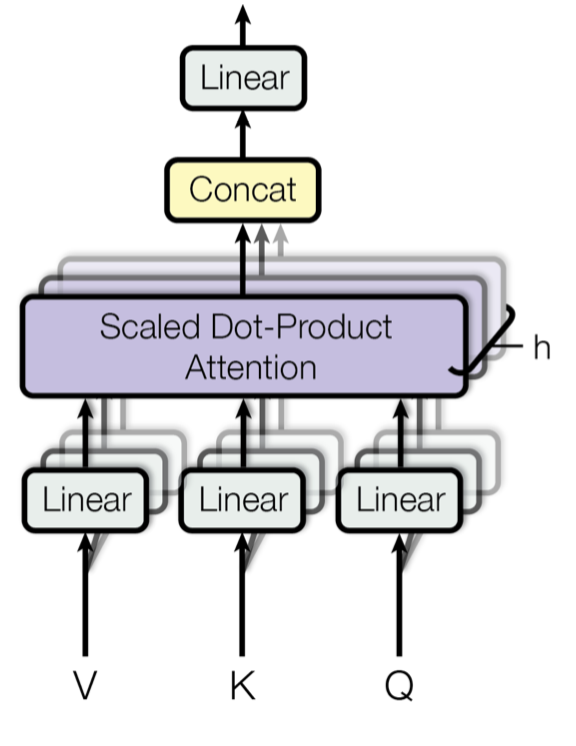
\includegraphics[width=80px]{img/transformer_11.png}\end{center}
  \end{textblock}

\end{frame}



\begin{frame}{Transformers in LLMs}
  \begin{textblock}{55}(4, 15)
    Transformers are essential in large language models (LLMs) due to their ability to process text sequences in a parallel and efficient manner

    \begin{itemize}
        \item \textbf{Encoding-Decoding} : Transformers use encoding layers to understand the context and decoding layers to generate text
        \item \textbf{Representation Learning} : LLMs learn rich representations of text by capturing long-term contextual relationship
    \end{itemize}

    \textbf{Transformer Architecture} : \\
    \begin{itemize}
        \item \textbf{Encoder} : Consists of multiple layers of attention and feed-forward networks
        \item \textbf{Decoder} : Similar to the encoder but with additional mechanisms for attention over the encoded input
    \end{itemize}
  \end{textblock}
  \begin{textblock}{35}(56, 28)
    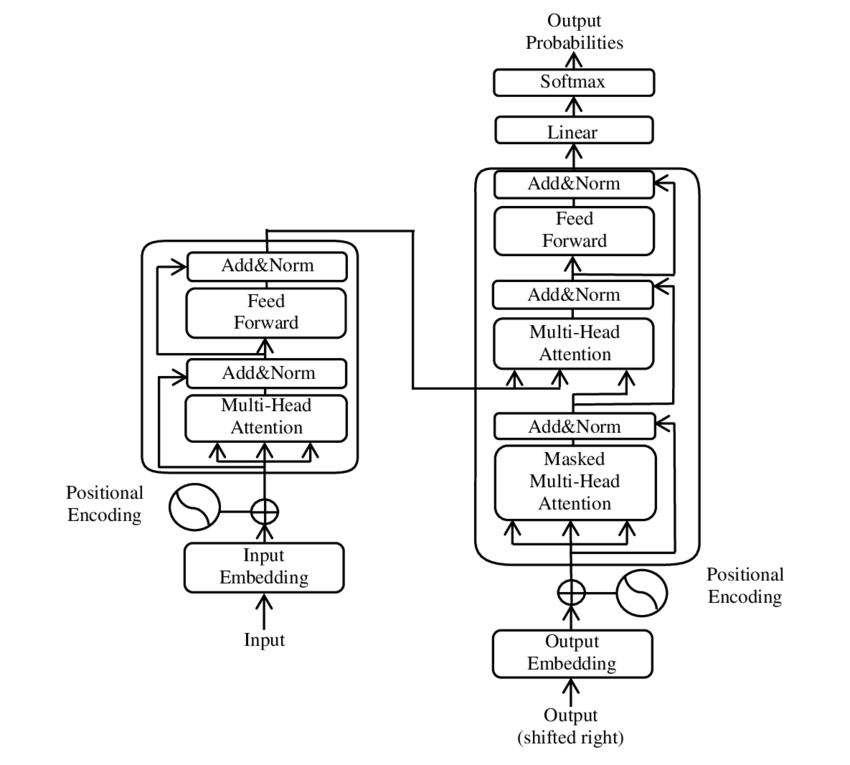
\includegraphics[width=170px]{img/transformer_architecture.png} % Make sure you have the image in the same folder or adjust the path.
  \end{textblock}
\end{frame}

\begin{frame}
  \frametitle{Transformers: other applications}
  \begin{itemize}
    \item Transformers have significantly impacted various fields beyond just NLP (image recognition, image generation, healthcare, autonomous vehicle, bioinformatics, etc)
    \item \textbf{AlphaFold 2 (Deepmind, 2021)}
  \end{itemize}

  \note{
    AlphaFold 2 is a groundbreaking artificial intelligence model developed by DeepMind that predicts the three-dimensional structures of proteins with remarkable accuracy.

    - Input and Data: amino acid sequence of a protein.  all the necessary information to determine the protein's structure
     multiple sequence alignments, to identify patterns and evolutionary information.

    - Attention Mechanism: The core of AlphaFold 2 is built on a deep learning architecture that employs an attention mechanism, similar to those used in language processing models like GPT-3. 
    
    This mechanism allows AlphaFold 2 to focus on specific parts of the protein sequence that are crucial for determining how the protein folds.

  }

  \begin{center}
    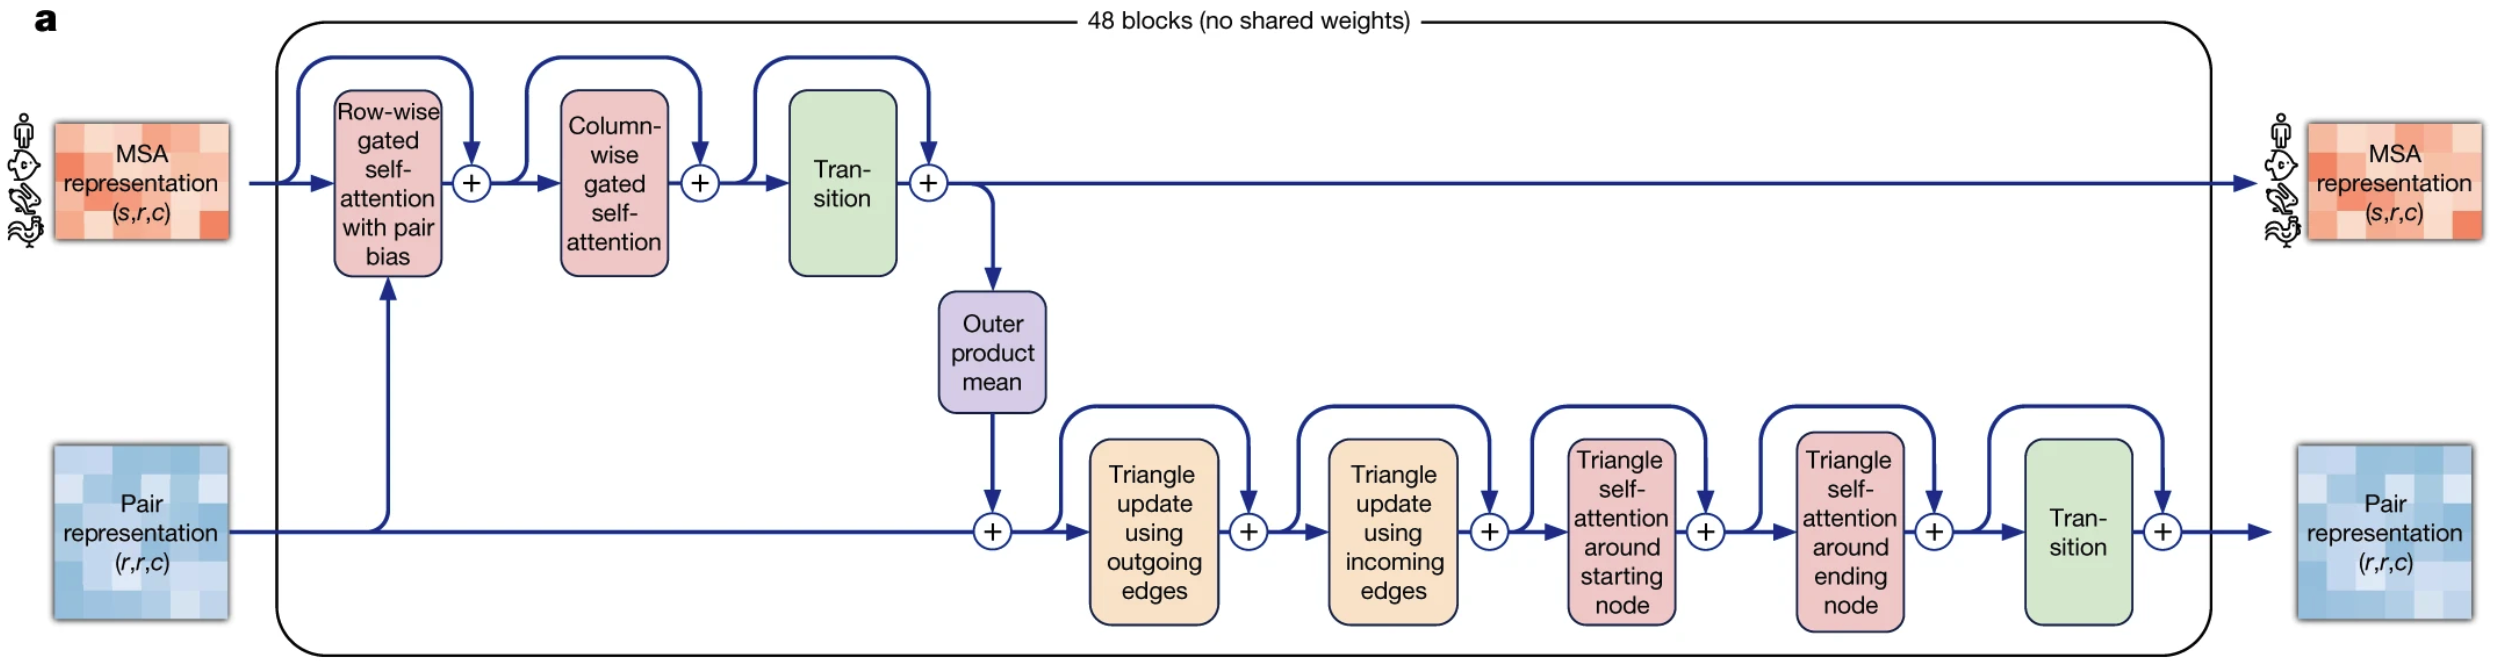
\includegraphics[width=200px]{img/alpha_fold_1.png}
    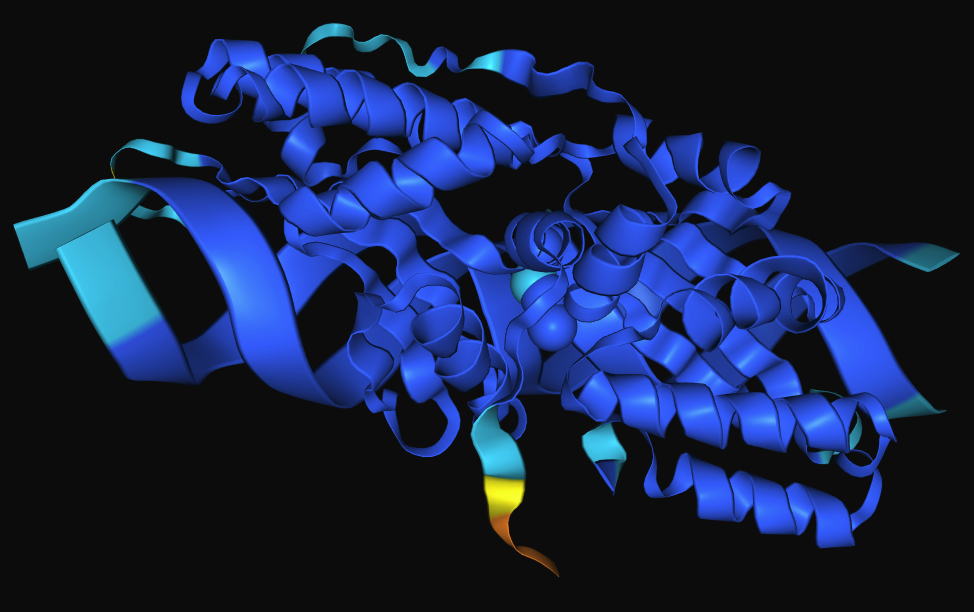
\includegraphics[width=110px]{img/alpha_fold_2.png}
  \end{center}
  

\end{frame}

\begin{frame}{Graph Neural Networks (GNNs)}
  \textbf{Geometric Deep Learning} \note{involves the study and development of deep learning models that can operate on non-Euclidean data such as graphs, manifolds, and other complex geometric structures}

  \begin{itemize}
      \item \textbf{Traditional Deep Learning} typically operates on Euclidean data (e.g., images, text)
      \item \textbf{Geometric Data} includes graphs, point clouds, and manifolds, which are not naturally represented in Euclidean space
  \end{itemize}

  \textbf{Graph Neural Networks} (GNNs) are a class of NN designed to perform inference on data described by \textbf{Graphs}: \note{They are particularly useful for tasks where the data is naturally represented as a graph structure.}
  \begin{itemize}
    \item \textbf{Nodes}: Represent entities in the graph.
    \item \textbf{Edges}: Represent relationships or interactions between entities
  \end{itemize}

\end{frame}

\begin{frame}{Graph Neural Networks (GNNs)}

  \note{
    \textbf{Key Components of GNNs}:
    \begin{itemize}
        \item \textbf{Node Embeddings}: Each node is represented by a feature vector
        \item \textbf{Aggregation}: Combining information from neighboring nodes
        \item \textbf{Update}: Non-linearly project aggregation to compute new node embeddings
        \item \textbf{Message Passing}: Nodes exchange information with their neighbors to update their embeddings
    \end{itemize}
  }
    \begin{center}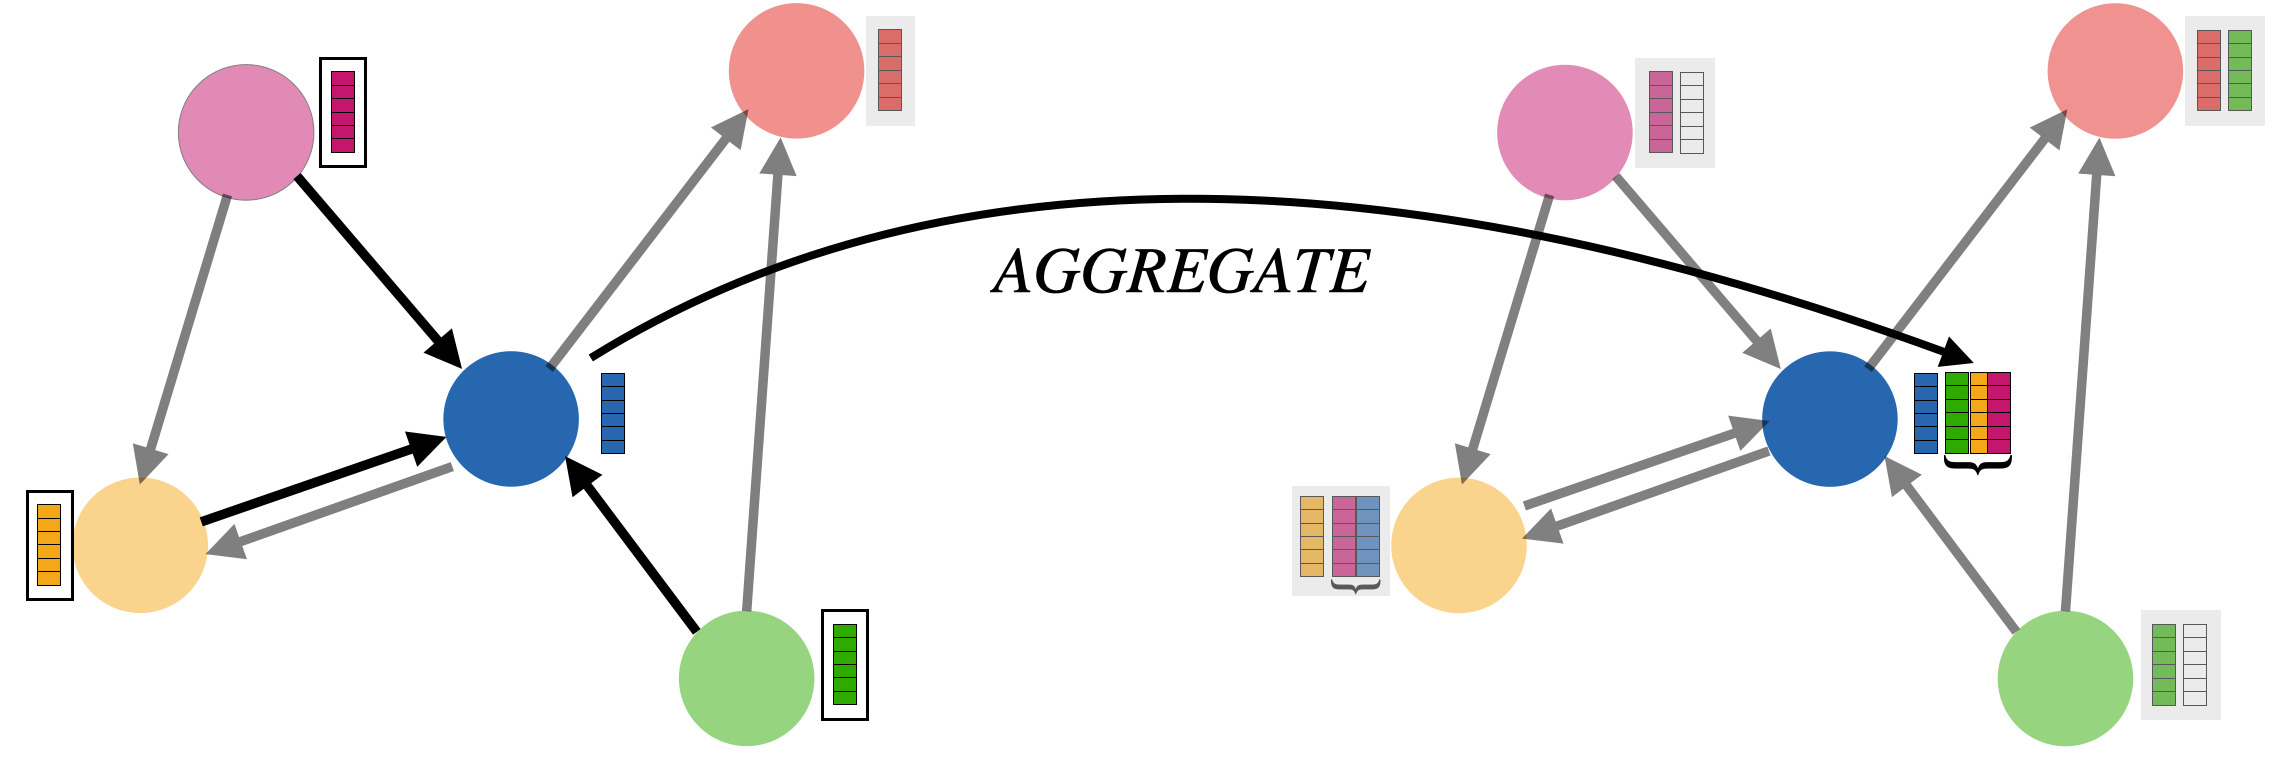
\includegraphics[width=200px]{img/gnn_aggregate.png}\end{center}
    \begin{center}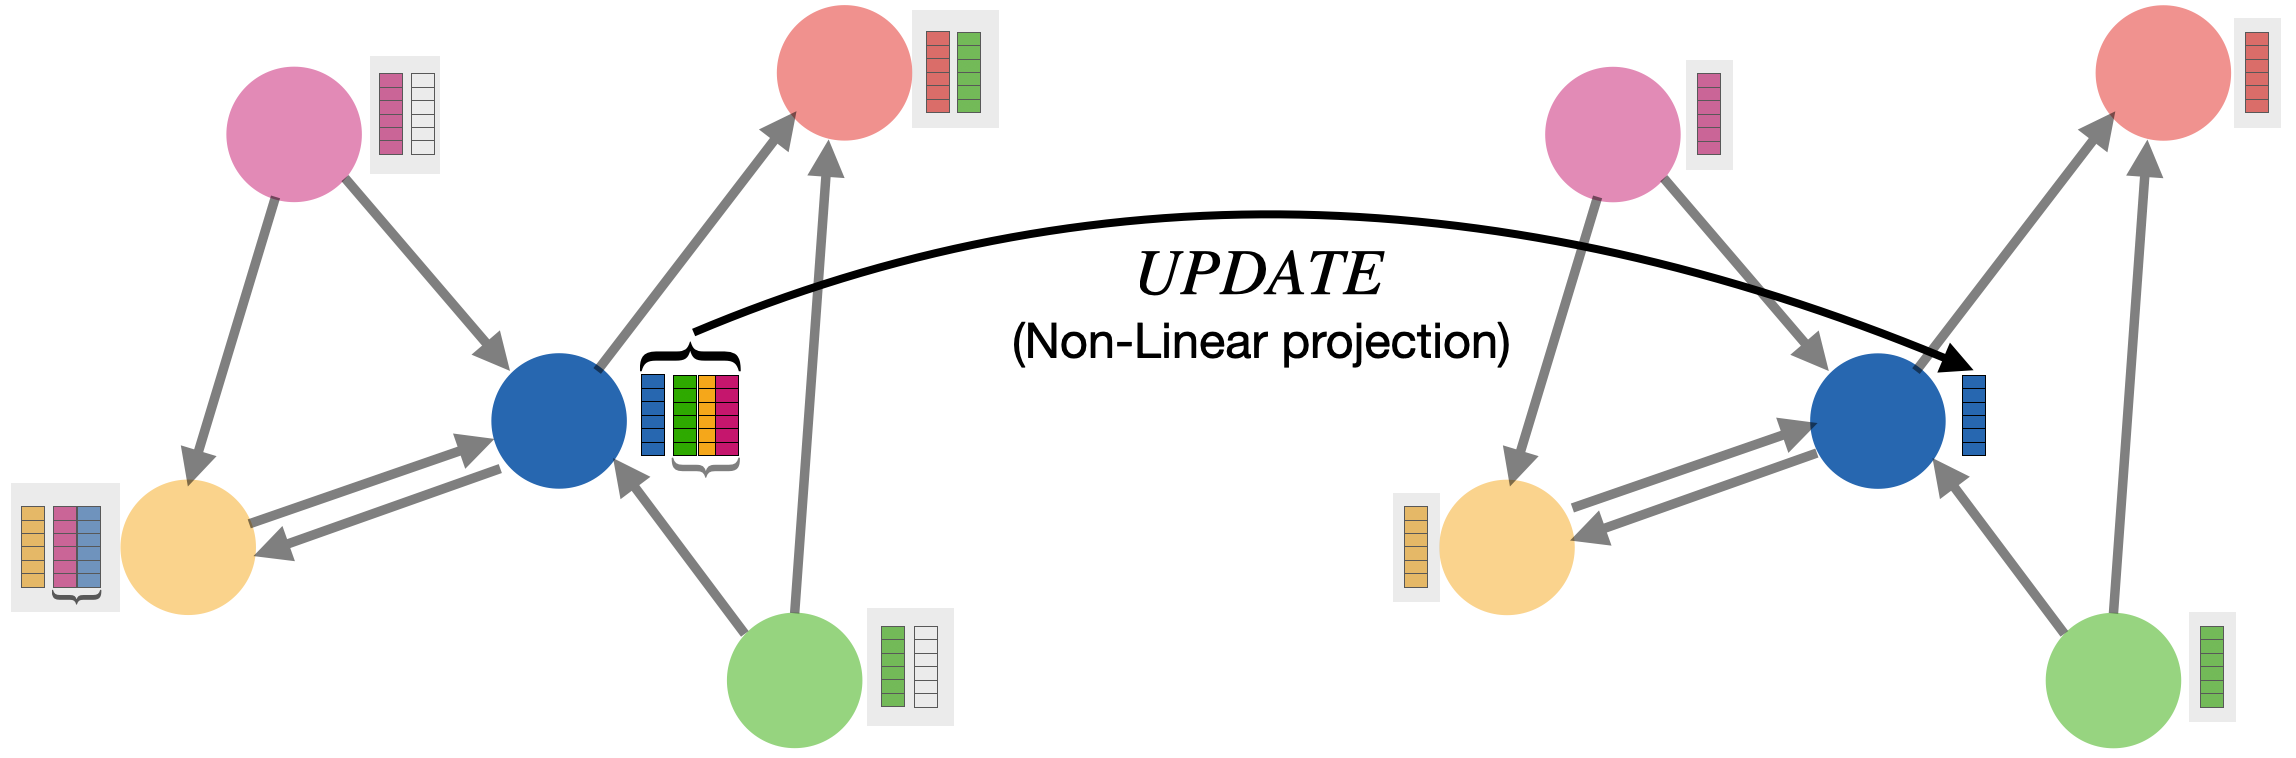
\includegraphics[width=200px]{img/gnn_update.png}\end{center}
  
  \textbf{Message Passing Formula}:
  \[
  h_i^{(k)} = \text{UPDATE}^{(k)}\left(h_i^{(k-1)}, \text{AGGREGATE}^{(k)}\left(\{h_j^{(k-1)} : j \in \mathcal{N}(i)\}\right)\right)
  \]
  where \(h_i^{(k)}\) is the embedding of node \(i\) at iteration \(k\), and \(\mathcal{N}(i)\) denotes the neighbors of node \(i\).

    \note{GNN can also be seenn as a generalization of convolution networks (Image seen as graphs) and transformers (sequence of text as a fully connected graph)}

\end{frame}

\begin{frame}
    \frametitle{Graph Neural Networks: applications}
    \begin{textblock}{90}(5, 15)
      \begin{itemize}
        \item Social Network analysis, Biological and Chemical Networks, Particle Physic, etc
        \item Widely used at LHC, GNNs especially suitable for sparse data of the detectors
        \item Geometric deep learning is a booming topic in AI 
      \end{itemize}
    \end{textblock}

    \begin{textblock}{40}(15, 45)
      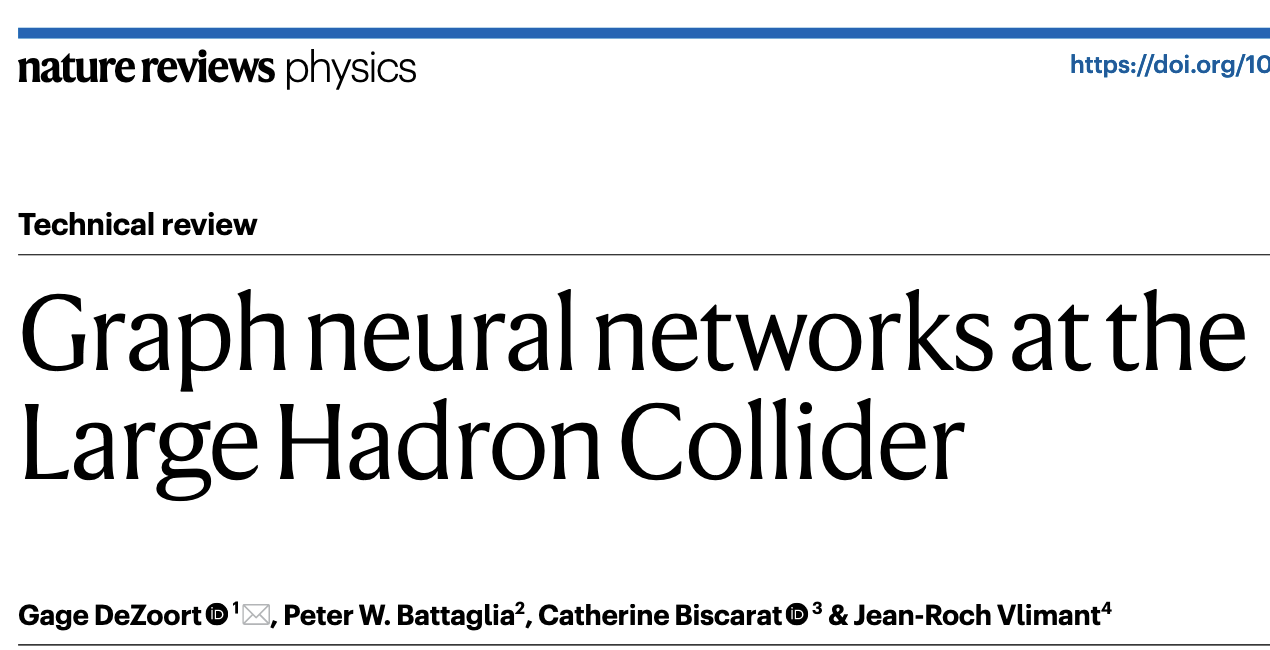
\includegraphics[width=140px]{img/gnn_lhc.png}
    \end{textblock}
    
    \begin{textblock}{30}(55, 40)
      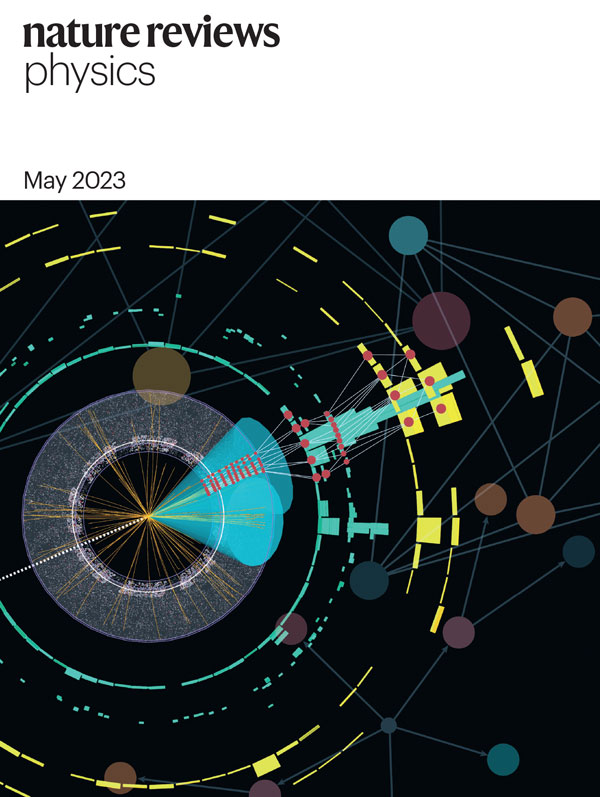
\includegraphics[width=110px]{img/gnn_lhc2.jpg}
    \end{textblock}

\end{frame}

%\subsection{New questions}

\begin{frame}
  \frametitle{GNN: an other interesting application example}
  \begin{textblock}{40}(2, 10)
    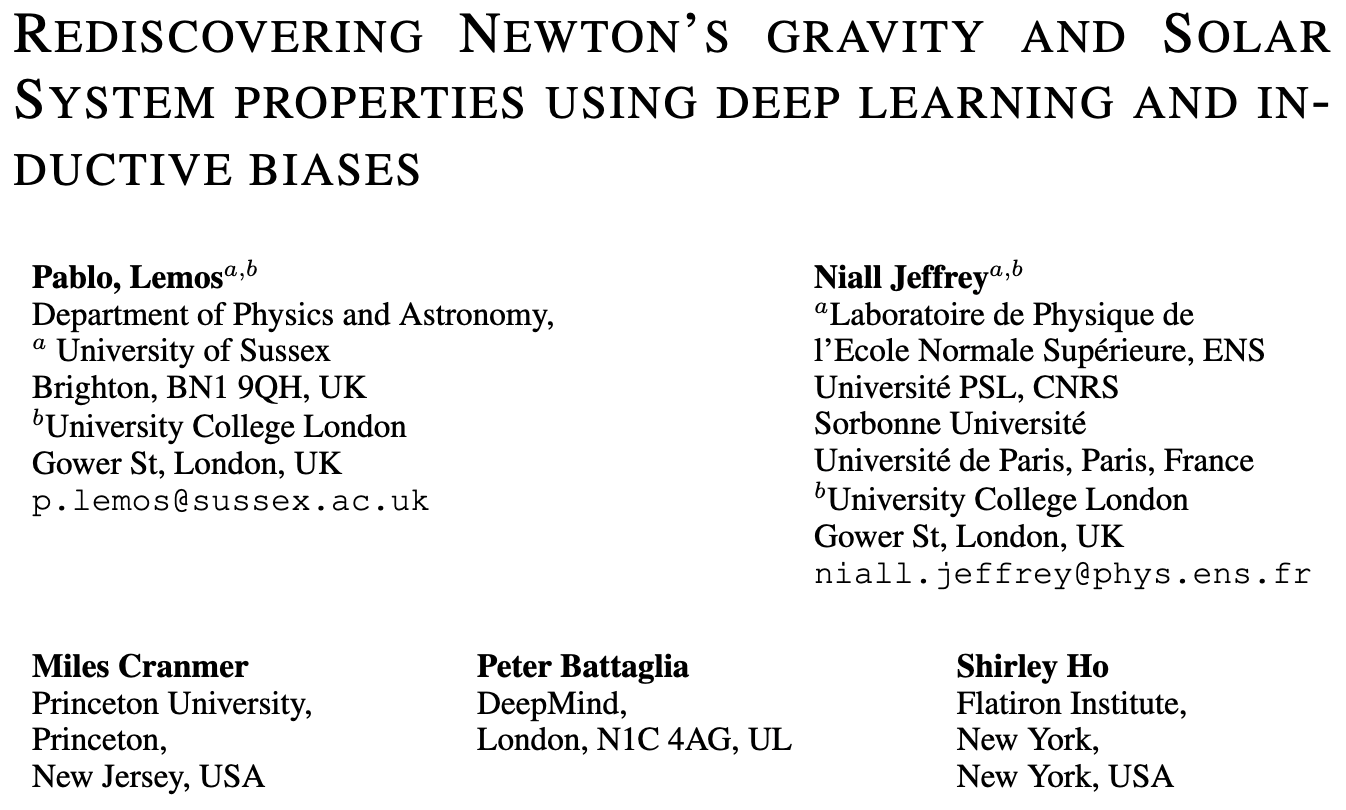
\includegraphics[width=150px]{img/retrieve_gravitation_laws_1.png}
  \end{textblock}
  \begin{textblock}{56}(44, 25)
    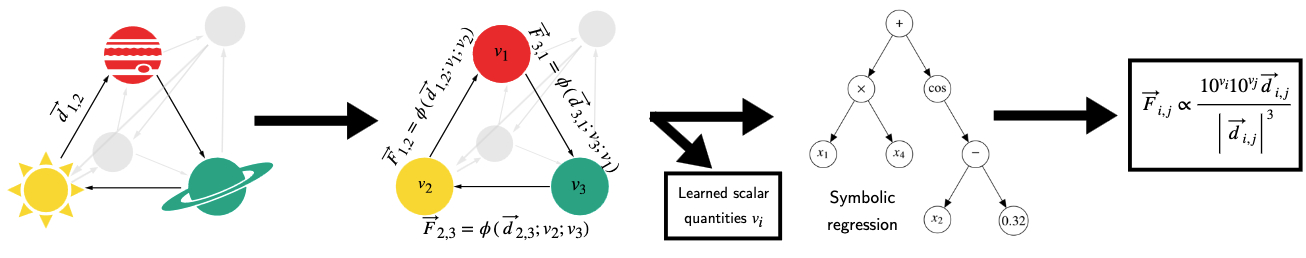
\includegraphics[width=200px]{img/retrieve_gravitation_laws_2.png}
  \end{textblock}
  \begin{textblock}{80}(4, 50)
    \begin{itemize}
      \item Based on GNN and symbolic regression
      \item Two-step approach: training a GNN-based simulator, then using symbolic regression to find analytical formulae for forces
      \item Loss function obtained by comparing this predicted acceleration and the true acceleration
    \end{itemize}
  \end{textblock}

  \note{By training a GN to simulate orbital
  dynamics from real data, authors say they were able to extract the edge function and correctly infer the formula
  for Newtonian gravitation.}

  \begin{textblock}{80}(4, 80)
    \begin{itemize}
      \item Do we want to automate Science? 
      \item What are the constraints and the theoritical limits? 
    \end{itemize}
  \end{textblock}

\end{frame}


\begin{frame}{AI now and tommorow in Science}
  \textbf{Combine Symbolic and Neural Networks} 
    \begin{itemize}
      \item \textbf{Combine NN and symbolic representations} \note{integrating a priori knowledge of the scientific domain}
      \item \textbf{Incorporating Prior Knowledge} \note{Embedding symbolic, pre-existing knowledge (like ontologies) into neural networks to guide learning}
      \note{\textbf{Enhancing Interpretability} Symbolic knowledge helps in making the models more interpretable and trustworthy}
      \item \textbf{Integration} of neuro-symbolic engine and multi-level representations
      \item \textbf{AlphaGeometry}
    \end{itemize}
  
  \textbf{Learn from heterogeneous data}
  \begin{itemize}
    \note{originating from various
    sensors in embedded systems (robotics, aerospace), from different detector subsystems /instruments or from different signal sources in a scientific
    experiment in general}
    \item Scientific data often \textbf{heterogeneous and multimodal} in nature
    \item \textbf{Learn shared latent representations}
    \item Enhance model's capacity to \textbf{represent} the data
    \item \textbf{Polymathic AI}
  \end{itemize}  


\end{frame}
